\documentclass[12pt, letterpaper]{article}
\usepackage[utf8]{inputenc}
\usepackage[spanish]{babel}
\usepackage{xcolor}
\usepackage{graphicx}
\usepackage{wallpaper}
\usepackage{amssymb}
\usepackage{pgf-pie}


\usepackage[colorlinks = true,
            linkcolor = black,
            urlcolor  = blue,
            citecolor = blue,
            anchorcolor = blue]{hyperref}
\graphicspath{ {Imagenes/} }

\setlength{\parindent}{10px}
\setlength{\parskip}{10px}
\renewcommand{\baselinestretch}{1.25}


\newcommand\BackgroundPic{%
\put(0,0){%
\parbox[b][]{\paperwidth}{
    \vfill
    \centering
    \vfill
    }}}
\begin{document}
\begin{titlepage}
    \ThisCenterWallPaper{1}{Imagenes/portada.jpg}
    \centering
    {\scshape\Large Universidad del País Vasco \par}
    {\scshape\Large Escuela de Ingeniería de Bilbao \par}
    \vspace{2cm}
    {\scshape\Huge {Documentación del proyecto} \par}
    {\itshape\Large Software de Gestión de Empresa\par}
    \vspace{5cm} 
    {\Large Bosco Aranguren \& Joel Bra \& Diego Marta\\Vicente Ayarza \& Natalia Martínez\par}
    \vspace{0.2cm}
    {\large Curso 2021/2022 \par}
    \vspace{0.1cm}
    
\includegraphics[scale=0.25]{Imagenes/logo.png}
\end{titlepage}
    
    
\thispagestyle{empty}
\clearpage
\tableofcontents
\clearpage
\section{Análisis del sector industrial
asignado}
El mercado de la informática se encuentra en una situación compleja. Por un lado la crisis del COVID y el teletrabajo supusieron un incremento en la demanda de ordenadores, mientras que por otro lado, la escasez de microprocesadores y los problemas de transporte internacional supusieron un decremento en la oferta. Esta situación plantea un horizonte con grandes oportunidades y riesgos para empresas del sector de la informática.


\subsection{Análisis del entorno competitivo (Porter)}
Usando las cinco fuerzas de Porter \textit{(Figura \ref{Porter})} podemos conocer el nivel de competencia que presenta un sector y determinar la estrategia que mejor se adapte a la situación. 

\begin{enumerate}
    \item \textbf{Amenaza de entrada de nuevos competidores potenciales:}
    
    Este apartado analiza la situación del mercado y las barrearas de entrada para nuevos competidores. En el montaje de ordenadores el producto principal por el que se paga son los componentes del ordenador más que el montaje de ellos. Debido a esto, este tipo de empresas tiene una gran parte que puede considerarse de distribución. Esto conlleva a que para poder ofrecer el mejor producto al mejor precio es necesario recibir las mejores ofertas de los proveedores. De esta característica surge la barrera de obtener componentes y dispositivos a buen precio y de gran variedad.

    \item \textbf{Amenaza de la aparición de productos sustitutivos:}
    
    En este apartado se analiza el riesgo de que un nuevo producto se haga con el mercado y sustituya el producto de nuestra empresa. Por el momento no parece posible la aparición de un producto sustitutivos del ordenador de sobremesa. Si bien los portátiles y tablets pueden llevarse una porción del mercado, ambos carecen de la capacidad y posibilidades que ofrece un ordenador de sobremesa y además ambos están disponibles como productos de nuestra empresa.

    \item \textbf{Poder de negociación de los proveedores:}
    
    Este apartado estudia el poder que tienen los proveedores a la hora de negociar los precios de los productos. En España existen muchos proveedores de componentes para ordenadores y artículos del sector de la informática. Esto es una ventaja para nosotros ya que evita que los proveedores pidan precios excesivamente altos por sus productos al tener que repartirse el mercado y ganar clientes. Como se ha mencionado en el primer apartado nos interesa tener una buena relación con nuestros proveedores y evitar que lideren las negociaciones de nuestras compras para lograr las mejores ofertas.

    \item \textbf{Poder de negociación de los clientes:}
    
    Similar al anterior apartado, este analiza el poder de negociación de los clientes sobre nuestro sector. Al igual que sucede con los proveedores, los clientes tienen un gran poder de negociación ya que España cuenta con muchas empresas que ofrecen nuestros productos y servicios. Para compensar esto debemos tener un gran representación web y ofrecer un sistema de compra online muy completo.

    \item \textbf{Rivalidad entre los competidores del sector:}
    
    El último apartado analiza las empresas rivales del sector. En España el sector esta principalmente compuesto por: PCComponentes, APP Informática, Aussar, Wipoid, Alternate y PCBox. Dependiendo de lo que el cliente busque cada una esta orientada a algo en especial (gaming, trabajo, componentes poco comunes, gamas...). Principalmente podemos dividir el mercado en dos categorías: online y física. Nuestra empresa se centrará en el mercado online ya que consideramos que nuestro producto principal no necesita de la presencia física del cliente sino de un buen servicio online.

\end{enumerate}
\section{Descripción de la empresa ficticia creada para el proyecto}
\subsection{Forma jurídica}
España cuenta con diferentes formas jurídicas para la correcta realización de la actividad económica, entre las que se ha elegido la Sociedad de Limitada (S.L.) por la siguientes razones:

\begin{itemize}
    \item No hay límite de socios que puedan participar.
    \item La inversión que se debe realizar es razonablemente pequeña (3.000€).
    \item La forma es jurídica, no física, indicando que la cantidad de dinero perdida en caso de empeoramiento de la situación financiera. Además, no existe un dueño como tal, por tanto, la responsabilidad recae en los socios.
    \item Los impuestos debidos a Hacienda, en caso de ser autónomo, pueden escalar en cuanto aumenten los ingresos. Sin embargo, el Impuesto de Sociedades, que se aplica en nuestro caso, escala hasta un máximo del 25\%.
\end{itemize}






\subsection{Estructura organizacional}
Existen diferentes tipos de estructuras organizacionales, entre las que elegiremos la estructura funcional. Esta forma cuenta con diferentes ventajas y desventajas que enumeraremos a continuación:

\begin{itemize}
    \item Cada empleado se encarga exclusivamente de sus tareas, aumentando la eficiencia y la productividad de cada trabajador.
    La supervisión de un área es más sencilla.
    \item La comunicación es mucho más directa al no haber intermediarios de por medio, ayudando a la eficiencia del equipo.
    \item Se reduce la presión sobre el individuo, ya que es más sencillo delegar y compartir responsabilidades.
    \item Pueden generar conflictos de autoridad y aumentar la rivalidad entre compañeros, ya que pueden intentar establecer su enfoque.
    \item Puede existir multiplicidad de objetivos, ocasionándose conflictos en las funciones generales de la organización.    
\end{itemize}

Nuestra empresa contará con un esquema donde el CEO (Chief Executive Officer) de la empresa es el cabeza de la junta directiva apoyado por los demás integrantes de la misma. De este departamento directivo colgarán los demás, que, a continuación, son detallados:

\textbf{Departamento de Marketing:} Es uno de los pilares más importantes de la empresa, debido a la necesaria promoción de la organización para darse a conocer, por ello, este departamento se integra en el resto de departamentos.

\textbf{Departamento de Recursos Humanos:} Este departamento gestiona todo lo relacionado con las personas que trabajan en la empresa. Podemos encontrar el área de contratación y formación del personal, dos de los objetivos más importantes del departamento. Nuestro departamento de Recursos Humanos estará formado por nuestro CHRO(Chief Human Resources Officer) cuya función es impulsar políticas de recursos humanos alineadas con los valores y estrategia de la empresa, y también contaremos con equipos de selección, formación y  gestión del personal.

\textbf{Departamento de Atención al Cliente:} Establece conexión entre la empresa y todos nuestros clientes post o pre compra, estableciendo una comunicación fluida mediante vía telefónica, por correo electrónico, mensajería o soporte técnico. Contaremos con un ATC manager, que será el encargado de asegurar un funcionamiento eficaz del departamento.

\textbf{Departamento de Logística y Almacén:} otro de los pilares más importantes de la empresa. Este departamento se encarga de guardar, proteger, conservar y enviar cada uno de nuestros productos que están en catálogo para su venta. Entre los objetivos del departamento destaca el mantenimiento de un servicio de gran calidad, garantizando la entrega al cliente en un servicio óptimo.

\textbf{Departamento de Postventa:} es el encargado de gestionar la garantía de los productos vendidos por nuestra empresa, ya sea relacionado con devoluciones, reparaciones o reembolsos. 

\textbf{Departamento de Compras:} analiza, evalúa y realiza la compra de los elementos necesarios para el funcionamiento de la empresa, eligiendo la calidad necesaria para cada momento y asegurando una gran calidad de los productos. Este departamento está directamente relacionado con una gran parte del resto de departamentos de nuestra empresa como pueden ser el de montaje o el de Logística y Almacén.

\textbf{Departamento de Mantenimiento y Mejora Continua:} desarrolla las funciones de mantenimiento preventivo y correctivo. A su vez busca obtener grandes cambios con pequeñas modificaciones consiguiendo un rendimiento más óptimo de la empresa.

\textbf{Departamento de Montaje:} nuestro departamento de montaje se divide en varias etapas, de cada una se encargará un grupo de trabajo especializado en ese área, optimizando el tiempo de producción y de entrega.

\subsection{Descripción de los productos ofertados}
Nuestra empresa oferta una serie de productos determinados:
\begin{itemize}
    \item Ordenadores Personalizados: Dentro de nuestra web ofrecemos la posibilidad de que el cliente elabore su propio ordenador con los componentes que el cliente crea más convenientes y que estén disponibles, aunque contará con unas recomendaciones sobré cuál es el componente más adecuado según su elección. A medida que añada componentes, se mostrará el coste del ordenador, sumándole un coste añadido por montaje. Una vez finalizado el proceso de configuración del ordenador personalizado, se pasará la información al departamento de montaje que se encargará de la realización del pedido. El ordenador contará con un seguro y servicio post-venta.
    \item Ordenadores:Hay disponibles en la web ordenadores portátiles y de sobremesa Cada ordenador tiene una descripción de las diferentes prestaciones del producto, por ejemplo, proveedor, componentes, precio, stock del producto. 
    \item Componentes: Otra sección de la web es la parte de componentes (periféricos y componentes de ordenador). Teniendo en cuenta que en la pestaña de ordenadores personalizados utilizan diferentes componentes para la creación de los ordenadores, esta pestaña y la de ordenadores personalizados comparten el mismo stock para evitar problemas de falta de stock. Además a cada componente se le tiene asociado su precio establecido.    
\end{itemize}
\subsection{Proveedores}
Para ejercer su labor, la empresa necesita un suministro continuado de componentes y periféricos para ordenador. Para obtenerlos se acudirá a las propias marcas o a otros mayoristas ya sea a nivel nacional o a nivel internacional, ya que la diversificación de proveedores es necesaria para reducir su nivel de negociación.

Por un lado destacaremos entre las propias marcas a MSI y ASUS, que serán las encargadas de abastecernos de los siguientes componentes para ordenador: tarjetas gráficas, placas base, cajas de ordenador y periféricos. Por otro lado, Intel y AMD nos venderán los procesadores, además del software para diagnóstico para empresas. En cuanto a los discos duros y otras memorias, tanto mecánicos como en esta sólido serán vendidos a nuestra empresa por Seagate. Finalmente, y terminando con las marcas, Corsair será la encargada de abastecernos de memoria ram, fuentes de alimentación y otros periféricos. A nivel nacional contamos también con Ordenadores Km0 que nos proporcionará todos los componentes para ordenador que necesitamos. Al ser un proveedor mayorista que tiene un almacén en territorio nacional, los tiempos de entrega podrían ser menores en algunos casos.

Finalmente, contamos con dos proveedores para los vinilos y la pintura que usaremos en los ordenadores personalizados. Por un lado, Leroy Merlin, y por otro, Ordenadores Km0. Ambos tienen almacenes con estos productos en territorio nacional, con lo que tendremos un buen tiempo de entrega.
\section{Diseño del sistema de gestión planteado para la empresa}
\begin{figure}[ht]
    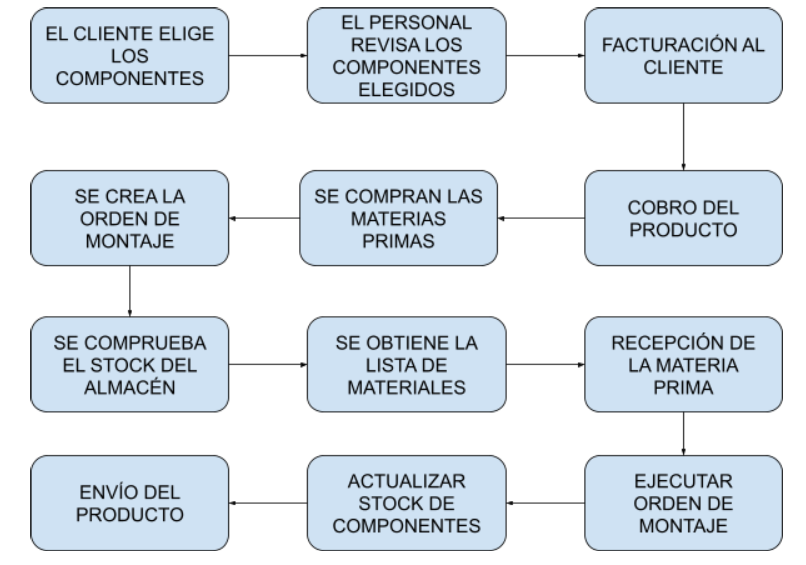
\includegraphics[width=\textwidth]{workflow.png}
    \caption{\textsf{Workflow del proceso de montaje de un ordenador}}
    \label{workflow}
\end{figure}
Explicación de cada proceso \textit{(Figura \ref{workflow})}:
\begin{itemize}
    \item \textbf{El cliente elige los componentes:} Es la acción que dará comienzo a la producción del ordenador que se va a montar. Aquí, el cliente elegirá los componentes que quiere dentro de su ordenador recibiendo sugerencias según su configuración. Una vez finalizado el proceso, se enviará al personal del departamento de montaje para la revisión.
    \item \textbf{El personal revisa los componentes elegidos:} El personal recibe la lista de componentes y periféricos dada por el cliente. Se asegura la correcta compatibilidad de todos los elementos. Si es correcta se pasará a la facturación del proyecto y, en caso negativo, se enviará al cliente un correo indicando las incompatibilidades.
    \item \textbf{Facturación al cliente:} Una vez esté todo correcto se procede a realizar la facturación; para ello se obtendrán los datos del cliente a facturar. Se determinan los productos a facturar, se establecen los posibles descuentos que haya y el medio de pago. Por último se indicará el plazo de pago.
    \item \textbf{Cobro del producto:} Se tramitará el cobro al cliente según el método de pago elegido, en caso de que no sea un cobro inmediato, se notificará al cliente sobre el plazo en el momento indicado.
    \item \textbf{Se compran las materias primas:} En primer lugar la detección de necesidad de compra, seleccionamos un producto y nos reunimos con el equipo de compras. Se especifica un presupuesto para la compra y se buscan proveedores.
    \item \textbf{Se crea la orden de montaje:} A la hora de crear una orden de montaje es necesario saber; el almacén desde el que saldrá la materia prima, el almacén destino, la cantidad de productos que se crearán y la selección del producto a crear.
    \item \textbf{Se comprueba el stock del almacén:} Se organiza, planifica y controla el conjunto de mercancías que hay en el almacén.
    \item \textbf{Se obtiene la lista de materiales:} Detallar los materiales precisos que se necesitan para la fabricación de un producto.
    \item \textbf{Recepción de la materia prima:} Se comprueba en qué estado llegan los productos así como la higiene del transporte y las instalaciones del proveedor.
    \item \textbf{Ejecutar orden de montaje:} Se ejecuta la orden creada anteriormente.
    \item \textbf{Actualizar stock de componentes:} Toma de datos de los activos, catalogación e inventario físico de activos con etiquetado y análisis de los registros.
    \item \textbf{Envío del producto:} La entrega debe realizarse de forma determinada y conforme a las condiciones establecidas en la compra.
\end{itemize}



\section{Checklist de elementos incluidos en el desarrollo}
\begin{itemize}
    \item \textbf{Producto distribuible:} Actualmente, la empresa cuenta con varios productos distribuibles, entre ellos, un portátil (Portátil ASUS X415EA - EB526) y los componentes que también usamos para el montaje de los ordenadores personalizados (procesadores, gráficas, discos duros…).
    \item \textbf{Producto fabricado que se planifica a través de un PMP:} La fabricación del ordenador personalizado Typhoon X1 se realiza mediante un programa maestro de la producción.
    \item \textbf{Producto fabricado just in time:} Cuando se pide un Backplate gráfica, se automatiza el proceso, creando la consecuente orden de producción y, en caso de ser necesario, una orden de compra para los materiales. Al tratarse de un producto JIT no se tiene inventario del mismo.
    \item \textbf{Producto tipo servicio que genera un proyecto:} Hemos creado el servicio \textit{Reparación de PCs} que, una vez un cliente nos lo pida, se generará el proyecto \textit{Reparar ordenador}.
    \item \textbf{Dos productos con variantes de dos atributos:} Contamos con dos ordenadores personalizados (Typhoon X1 y Cycloon X1), los cuales tienen cuatro variantes que juntan un vinilo y una pintura. Por ejemplo, existe el PC Typhoon X1 con vinilo moderno y pintura azul, pero también existe el mismo ordenador con vinilo de videojuego y pintura azul.
    \item \textbf{Lista de materiales de, al menos, 3 materias primas en los productos fabricables:} Los ordenadores personalizados (Typhoon X1 y Cycloon X1) cuentan con ocho listas de materiales diferentes entre los dos debido a las variantes creadas. De todas formas, en todas las listas se mostrarán los 7 componentes diferentes para cada modelo pero iguales entre variantes del producto.
    \item \textbf{Jerarquías de productos:} Se han creado categorías para todos los productos de la empresa. Todos los componentes utilizados estarán en la categoría de componentes, dentro de ella, hay diferentes categorías para cada tipo de producto (disco duro, gráfica, torre…) y, finalmente, la categoría procesadores, por ejemplo, estará dividida en Intel y AMD. Las categorías también se usan para los productos fabricados y los elementos de decoración.
    \item \textbf{Dos tarifas en los productos que se compran:} Cada producto que se compra cuenta con dos tarifas con diferentes tarifas y cantidad de producto que se debe comprar. Generalmente, tendremos a Ordenadores Km0, que nos ofrecerá mejores tiempos de envío pero peores precios, y a la empresa fabricante (Intel, AMD, Asus…) que nos ofrecerán mejores precios pero, al tener almacenes fuera del estado, peores tiempos de envío.
    \item \textbf{Tarifas de venta:} Se han creado dos tarifas diferentes para nuestros productos en venta. Por un lado, tenemos la \textit{Tarifa pública}, que se aplicará a particulares y, por otro, tenemos la \textit{Tarifa empresas}, que se aplicará a empresas y ofrece un descuento con respecto de la pública puesto que las compañías realizan pedidos más grandes.
    \item \textbf{Equipos de venta:} La empresa cuenta con dos equipos de venta que desempeñarán diferentes funciones dentro del departamento. El equipo Ventas de \textit{PCs personalizados} se encargará de la gestión de los pedidos relacionados con los productos fabricados. Tendrá como miembros a Diego Marta (gerente), María Salazar, Martín Marta y José Antonio Pérez. Por otro lado, el equipo de \textit{Ventas de portátiles} se encargará de gestionar los pedidos de portátiles y otros componentes. Estará compuesto por Vicente Ayarza (gerente), Juan Segura, David Carral y Felipe Amaya.
    \item \textbf{Oportunidades de venta, pedidos en fase de presupuesto y ventas confirmadas:}
    \begin{itemize}
        \item \textbf{Oportunidades de venta:} Las oportunidades de venta creadas se encuentran en diferentes fases:
        \begin{itemize}
            \item \textbf{Nuevas:} Oportunidad Sport Medicine Castro (encargada a Diego Marta y con una tarea de envío de email) y Oportunidad de AMD (encargada a Vicente Ayarza y con una tarea de llamada).
            \item \textbf{Calificadas:} Oportunidad de MediaMarkt España (encargada a Diego Marta y con una tarea de llamada).
            \item \textbf{Propuesta:} Oportunidad de Jose Antonio Musk (encargada a David Carral).
            \item \textbf{Ganado:} Oportunidad de Juan José Zamora (asignada a Vicente Ayarza) y Oportunidad de Frutería Jesús (asignada a Juan José Zamaro).
        \end{itemize}
        \item \textbf{Pedidos en fase de presupuesto:} 
        \begin{itemize}
            \item S00002 (asignado a José Antonio Pérez con tarea de propuesta).
            \item S00003 (asignado a Juan Segura con tarea mandar presupuesto).
            \item S00010 (asignado a Vicente Ayarza).
            \item S00005 (asignado a Diego Marta con tarea de llamada cliente).
            \item S00009 (asignado a José Antonio Pérez con tarea mandar presupuesto).
            \item S00013 (asignado a Vicente Ayarza con tarea propuesta presupuesto).

        \end{itemize}
        \item \textbf{Ventas confirmadas:} existen más de 5 pedidos entre los que destacaremos S00001, S00004, S00006, S00008 y S00011.
    \end{itemize}
    \item \textbf{Descuentos en la línea de pedido:} Se han descuentos en los pedidos S00014 (10\%) y S00009 (15\%).
    \item \textbf{Costes de envío en función de la zona geográfica:} Se han creado tres tarifas de envío: el envío estándar, que se aplica a Andorra, España, Francia y Portugal; el envío a islas, que se aplica a las Islas Baleares y a las Islas Canarias; y el envío resto Europa, que se aplica a Alemania, Austria, Eslovaquia, Grecia, Holanda, Italia y la República Checa.
    \item \textbf{Órdenes de producción:} existen 5 órdenes de producción de PC Typhoon X1 y de PC Cycloon X1 (WH/MO/ 00003 (hecha), WH/MO/ 00004 (hecha), WH/MO/00005 (en progreso), WH/MO/00006 (confirmado), WH/MO/00007 (confirmado)).
    \item \textbf{Órdenes de compra:} Se han creado varias órdenes de compra entre las que destacan las siguientes: P00001 (Ordenadores Km0 encargado a Bosco Aranguren), P00002 (ASUS encargado a Lucas Gomez), P00003 (Corsair encargado a Bosco Aranguren), P00004 (Leroy Merlin España encargado a Jesús Rasines) y P00005 (Intel encargado a Bosco Aranguren).
    \item \textbf{Tareas del proyecto Reparar Ordenador:} Recepción del ordenador (departamento de almacén), búsqueda de problemas (departamento de montaje), búsqueda de herramientas (departamento de montaje), búsqueda de componentes necesarios (departamento de montaje), reparación (departamento de montaje), embalaje (departamento de almacén).
    \item \textbf{Etapas de ejecución del proyecto Reparar Ordenador:} las tareas que contienen este proyecto son Nuevas órdenes, Juntar materiales, Arreglar ordenador, A enviar.
    \item \textbf{Ventas de producto tipo servicio:} S00004 y S00005, con diferentes tareas a lo largo de las tareas del proyecto.
    \item \textbf{Horas de trabajo:} se han agregado las horas de trabajo de los empleados que han realizado sus tareas diariamente, como se puede ver en el caso de Joel Bra.
    \item \textbf{Permisos:} se han ajustado los permisos a los trabajadores dependiendo del rol que tengan en el departamento y en la empresa.
    \item \textbf{Informes:}
    \end{itemize}

    Compras por proveedor:  

    \begin{tikzpicture}
            \pie{4/ASUS,
            10/Corsair,
            6/Intel,
            58/Leroy Merlin,
            4/MSI Gaming,
            18/Ordenar KM0}
    \end{tikzpicture}

    Compras por país de origen: 
    
    \begin{tikzpicture}
            \pie{20/Estados Unidos,
            70/España,
            7/Italia,
            3/Taiwan}
    \end{tikzpicture}
    
    


\section{Bibliografía}
\href{https://www.esan.edu.pe/conexion-esan/la-estructura-organizacional-funcional#:~:text=La%20estructura%20funcional%20es%20la,%2C%20producci%C3%B3n%2C%20ventas%2C%20etc.}{Esan.edu \textit{La estructura organizacional funcional}}

\href{http://www.ipyme.org/es-ES/DecisionEmprender/FormasJuridicas/Paginas/FormasJuridicas.aspx}{IPYME, \textit{Formas Jurídicas}}


\href{https://www.thepowermba.com/es/blog/las-5-fuerzas-de-porter#:~:text=Como%20hemos%20indicado%2C%20las%20cinco,sustitutivos%20y%20rivalidad%20entre%20competidores.}{The power MBA, \textit{Las 5 fuerzas de Porter: análisis de las fuerzas competitivas de una empresa}}
\end{document}